\section{Devices Used}

For the purposes of evaluating the performance of both the scorer and the scorer
and parser, a Mac Pro (Early 2008 - MacPro3,1) was used. This was fitted with
two Intel Xeon E5462 processors, and a nVidia Tesla C2075 GPU. In addition,
there was a separate machine fitted with an Intel Xeon Phi 5110P. An AMD system
with a traditional CPU setup with 4x AMD Operon 6366 HE CPUs was also used. A
brief overview of the hardware will be given to provide some perspective to the
results which follow.

\subsection{Mac Pro System}

The Mac Pro was running Mac OS X version 10.8.5 (Build Version 12F45). Both the
nVidia and Intel OpenCL SDKs were installed and up to date at time of writing.

\begin{description}

\item[CPU] The motherboard has two CPU sockets, both with an Intel Xeon E5462
\footnote{\url{http://ark.intel.com/products/33084/Intel-Xeon-Processor-E5462
-12M-Cache-2_80-GHz-1600-MHz-FSB}} processor. This is a quad core processor with
a 2.8GHz clock speed and 12MB of Level 2 cache per processor.

\item[Primary Memory] There is 14GB of PC2-6400 (800MHz) DDR2 RAM installed,
with error correcting code (ECC) enabled.

\item[GPU] The GPU is an nVidia Tesla C2075
\footnote{\url{http://www.nvidia.co.uk/docs/IO/43395/NV-DS-Tesla-C2075.pdf}}.
The device has 6GB of dedicated GDDR5 memory running at 1.5GHz giving an
internal memory bandwidth of 144GB/s. There are 448 ``CUDA Cores'' with a clock
frequency of 1.15GHz. It has been installed in a PCIe 1.0 slot with 16x lane
bandwidth giving a total theoretical bandwidth between its on-board memory and
main memory of 4GB/s (250MB/s per lane).

\end{description}

\subsection{Intel Xeon Phi System}

The system is running the SUSE Enterprise Server 11 Linux distribution. This
system was used for running the software system on the Intel Xeon Phi. There are
two Intel Xeon Phis fitted and these were used to investigate the performance of
a single and a dual Intel Xeon Phi set up. The system does not have a graphics
card fitted.

\begin{description}

\item[CPU] There is a single Intel Xeon E5-2620
\footnote{\url{http://ark.intel.com/products/64594/intel-xeon-processor-e5-2620
-15m-cache-2_00-ghz-7_20-gts-intel-qpi}} fitted. This is a six core processor
with hyper-threading to give twelve hardware threads. The standard clock
frequency is 2GHz with a maximum turbo frequency of 2.5Ghz. There is a total of
15MB ``Intel Smart Cache'' available which acts as Level 3 cache.

\item[Primary Memory] 16GB DDR3 RAM

\item[Intel Xeon Phi] The Intel Xeon Phi is the 5110P
\footnote{\url{http://ark.intel.com/products/71992/intel-xeon-phi-coprocessor-
5110p-8gb-1_053-ghz-60-core}} variant. There are sixty physical CPU cores
running at 1.053GHz, the cores are 4-way hyper-threaded resulting in 240
hardware threads. There is 8GB of on board memory running at 5GT/s for a
theoretical maximum memory bandwidth of 320GB/s. It has been installed in a PCIe
2.0 slot with 8x lane bandwidth giving a total theoretical bandwidth between
its on-board memory and main memory of 4GB/s (500MB/ per lane).

\end{description}

\subsection{AMD System}

The system is running the Fedora 18 Linux distribution. This system was used
solely for running the software system on the AMD CPUs and does not have a
graphics card fitted.

\begin{description}

\item[CPU] There are four AMD Opteron 6366 HE
\footnote{\url{http://products.amd.com/en-us/OpteronCPUDetail.aspx?id=813&f1=&f2
=&f3=Yes&f4=&f5=&f6=&f7=&f8=&f9=&f10=&f11=&}} (high efficiency) processors
fitted. Each processor has 16 cores running at a base clock speed of 1.8GHz with
a maximum turbo frequency os 3.1GHz. There is 1MB of Level 2 and 16MB of Level 3
Cache available per processor.

\item[Primary Memory] 512GB DDR3 RAM

\end{description}

\section{Experiment Set up and Input Files}

\subsection{Data Transfer}

The first experiment conducted was to investigate the effect of the PCI Express
bus transfer rate on overall system performance. The classification system
involves the transfer of very small (4KB) OpenCL buffers, up to very large (100s
of MB and above) OpenCL buffers. Both present potential performance concerns.
Small transfers can result in low throughput as the waking up of the PCI Express
bus and setting up of data transfer can overshadow the actual transfer time.
Large transfers, even though being they may be being transferred at the maximum
possible transfer rate, will, due to their size, take up significant amount of
time to transfer. If the transfer time is significant in regards to the actual
time to score the transferred documents, use of an accelerator device could be
inefficient, irrespective of the processing power of the accelerator.

There are currently four PCI Express bus standards in place, the first two are
in use in the systems discussed above. Each standard doubles (or nearly doubles)
the theoretical maximum bandwidth of a single PCI-E lane in each direction.
Table~\ref{table:pciE} shows this alongside the sampling rate in gigatransfers
per second (GT/s) and encoding of data.

\begin{table}[H]
\begin{tabular}{|l|l|l|l|l|}
\hline
PCI-E Standard & Sampling rate per lane & Data encoding & Single lane speed &
Sixteen lane speed\\
\hline
PCI-E 1.0 & 2.5 GT/s & 8b/10b & 250MB/s & 4GB/s\\
\hline
PCI-E 2.0 & 5 GT/s & 8b/10b & 500MB/s & 8GB/s\\
\hline
PCI-E 3.0 & 8GT/s & 128b/130b & 985MB/s & 15.75GB/s\\
\hline
PCI-E 4.0 & 16GT/s & 128b/130b & 1969MB/s & 31.51GB/s\\
\hline
\end{tabular}
\caption{PCI-E Bus Speeds (each direction)}
\label{table:pciE}
\end{table}

As Table~\ref{table:pciE} shows, theoretical bandwidth nearly doubles on each
iteration. The change from 8b/10b encoding, with 20\% transfer overhead, to
128b/130b encoding, with around 1.56\% transfer overhead, allowed an increase in
of bandwidth of nearly 100\% even though the sampling rate only increased by
60\%.

The Mac Pro system connects the Tesla C2075 to a sixteen lane PCI-E 1.0 slot and
the Intel Phi system connects the Intel Xeon Phi to an eight lane PCI-E 2.0 slot
which theoretically has the same bandwidth as the sixteen lane PCI-E 1.0 slot.

nVidia's CUDA SDK supplies a bandwidth test which was used to determined the
bandwidth of the Mac Pro system. The tool, called ``bandwidthTest'' has a mode
which is referred to as ``shmoo'' that runs a series of tests of increasing
size, from 1KB up to 64MB to give the full range of possible values.

\subsection{Document Classification}

For each device, the system (scoring only or scoring and parsing) was run over a
number of different profiles. There are twelve profiles in total, each 128MB in
size. The twelve profiles each had a different combination of terms relating to
the two classes a document could come under. Given that the profile is the same
size, the profiles themselves do not affect performance, only the classification
of documents. Each profile run would be repeated several times.

For the scoring only system, a pre-parsed collection of terms for the TREC
collection is given. The parser and scoring only system receives the original
TREC collection text file. The TREC collection is a 236MB text file containing
77876 documents in plain text. Each document is enclosed by DOC tags and
contain a document number, a date and time, a category, headline, and a series
of paragraphs for the document itself.

Each device is given three different bloom filter inputs. The first is the
``normal'' bloom filter. This bloom filter is actually generated from the
profiles and will result in the same classification as the non bloom filter
runs.

The second is the ``all hits'' bloom filter. This bloom filter is created to be
completely full and thus always result in a hit, irrespective of whether or not
the term is in the profile. This is seen as a worst-case scenario performance-
wise when running with a bloom filter, the case where no reads from main memory
are prevented. This will result in the same classification as the non bloom
filter runs.

The third is the ``no hits'' bloom filter. This bloom filter is created to be
completely empty and thus never results in a hit, irrespective of whether or not
the term is in the profile. This is seen as a best-case scenario performance-
wise when running with a bloom filter, the case where all reads from main memory
are prevented. This results in a completely zero score classification for all
documents however, alongside the ``all hits'' bloom filter, results in a range
of performance values possible when using a bloom filter.

\section{Data Transfer Results}

Figure \ref{fig:dataTransfer} shows the data transfer speeds between host and
device on the Mac Pro system. The theoretical maximum bandwidth of the system is
4GB/s and, with large enough transfers, around 3.2GB/s (80\% of theoretical)
is achieved.

Transfers that are less than 100 kilobytes, for instance the 4KB bloom filter,
suffer very low transfer speeds, with the bloom filter being transferred at
around 850MB/s. With the next smallest buffer to be transferred being on the
order of hundreds of kilobytes (scoring results), the slow transfer rate is
not going to cause significant impact on overall performance.

\begin{figure}[H]
\centering
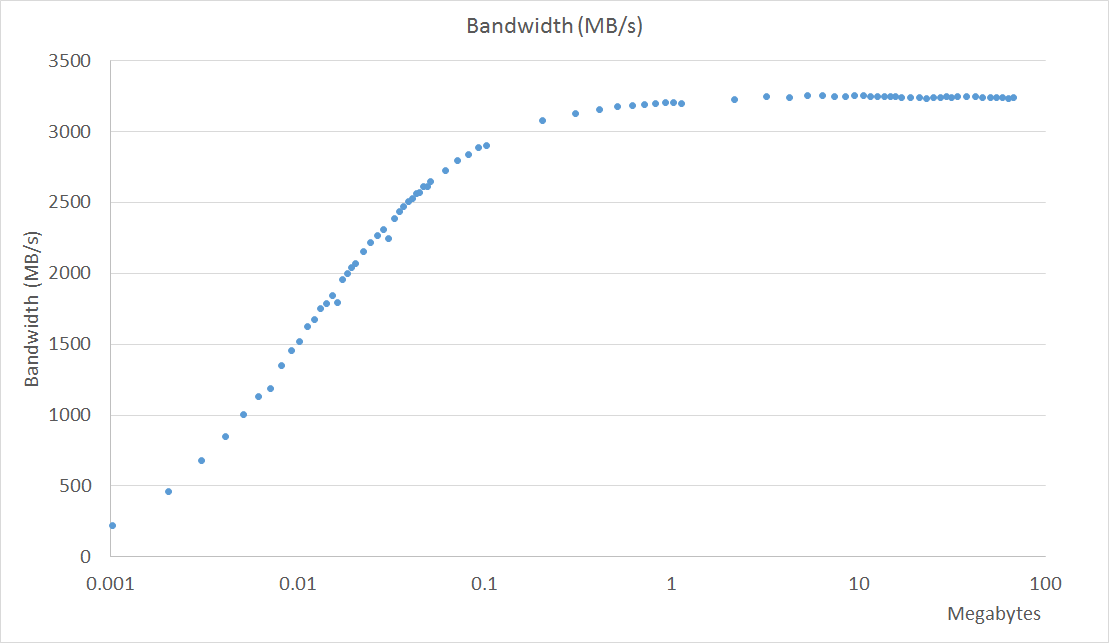
\includegraphics[width=\linewidth]{images/faraBandwidth.png}
\caption{PCI Express bus transfer rates}
\label{fig:dataTransfer}
\end{figure}

\section{Scoring Only Results}

This experiment is to investigate how well GPUs score documents, having been
given a parsed document set. Scoring is a highly parallel task thus GPUs are
suited for this kind of task.

Table \ref{table:scoringOnly} contains the results from the scoring only
experiments. The results are the average time and throughput of the system over
the twelve profiles.

Each profile run is repeated ten times to improve the accuracy and reliability
of the timing mechanism. The exception to this rule is the AMD system which,
due to its significantly higher throughput, required one hundred repetitions
per profile to achieve reliable results.

The C++ Single Threaded and C++ Multi-threaded results are there for reference
and to indicate how effective parallelism is for document filtering.

\begin{table}[H]
\begin{tabular}{|l|l|l|l|}
\hline
Device & Test & Time (ms) & Throughput (MB/s)\\
\hline
\multirow{4}{*}{2x Intel Xeon E5462 C++ Single Threaded}
& No Bloom Filter & 2537 & 93 \\
& Bloom Filter & 2617 & 90.2 \\
& Bloom Filter All Hits & 4023 & 58.7 \\
& Bloom Filter No Hits & 2006 & 117.4 \\
\hline
\multirow{4}{*}{2x Intel Xeon E5462 C++ Multi-threaded}
& No Bloom Filter & 390 & 605.1 \\
& Bloom Filter & 336 & 702.4 \\
& Bloom Filter All Hits & 550 & 429.1 \\
& Bloom Filter No Hits & 257 & 918.3 \\
\hline
\multirow{4}{*}{2x Intel Xeon E5462 OpenCL}
& No Bloom Filter & 222 & 1063.1 \\
& Bloom Filter & 156 & 1512.8 \\
& Bloom Filter All Hits & 298 & 791.9 \\
& Bloom Filter No Hits & 104 & 2269.2 \\
\hline
\multirow{4}{*}{nVidia Tesla C2075}
& No Bloom Filter & 258 & 914.7 \\
& Bloom Filter & 232 & 1017.2 \\
& Bloom Filter All Hits & 294 & 802.7 \\
& Bloom Filter No Hits & 216 & 1092.6 \\
\hline
\multirow{4}{*}{Intel Xeon Phi 5110P}
& No Bloom Filter & 381 & 619.4 \\
& Bloom Filter & 409 & 577 \\
& Bloom Filter All Hits & 456 & 517.5 \\
& Bloom Filter No Hits & 402 & 587.1 \\
\hline
\multirow{4}{*}{4x AMD Opteron 6366 HE}
& No Bloom Filter & 87 & 2712.6 \\
& Bloom Filter & 50 & 4720 \\
& Bloom Filter All Hits & 96 & 2458.3 \\
& Bloom Filter No Hits & 39 & 6051.3 \\
\hline
\end{tabular}
\caption{Scoring Only Results}
\label{table:scoringOnly}
\end{table}

Figure \ref{fig:scoringOnlyBest} takes each device's best result and compares
them in a bar graph. The AMD system has the clear lead, having nearly three
times the performance of the second fastest system. It's important to note
however that these figures are only used for reference. There would need to
be some part of the system conducting the parsing section.

\begin{figure}[H]
\centering
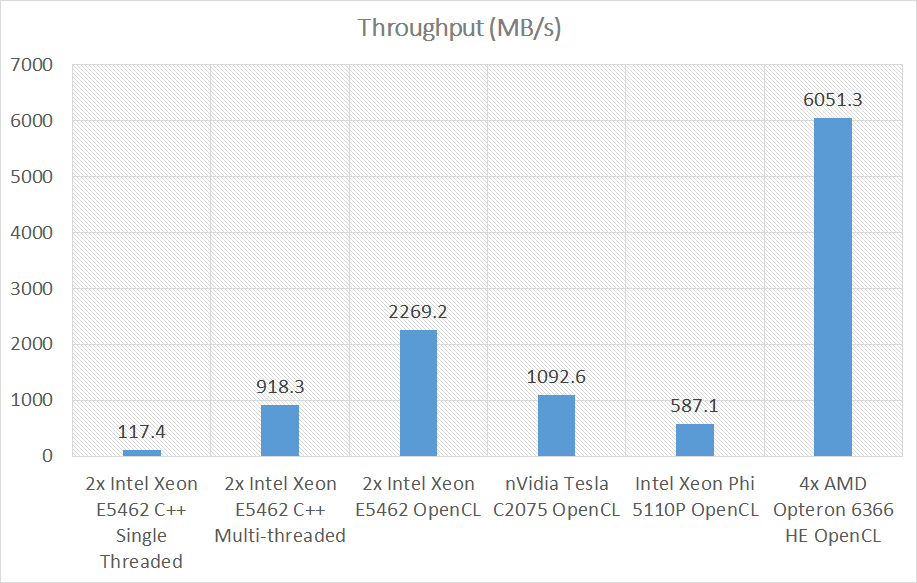
\includegraphics[width=\linewidth]{images/scoringOnlyBest.png}
\caption{Scoring Only Device Comparison}
\label{fig:scoringOnlyBest}
\end{figure}

\section{Parsing and Scoring Results}

Having shown that scoring on the GPU is faster than the parsing on the CPU
(427MB/s \cite{HybridCPUFPGA}), the parsing and scoring experiment was set up
to investigate if GPUs and the Intel Xeon Phi was suitable for both parsing
and scoring, in an attempt to remove the CPU parsing bottleneck.

Table \ref{table:parsingScoring} contains the results from the parsing and
scoring experiments. The results are the average time and throughput of the
system over the twelve profiles.

Each profile run is repeated ten times to improve the accuracy and reliability
of the timing mechanism. The exception to this rule is the Intel CPU and nVidia
GPU system which, due to the fact that both devices were running in parallel and
run at slightly different rates, required different numbers of repetitions to
finish at the same time. The ``No Bloom Filter'' experiment required twenty
repetitions in total (ten for each device), ``Bloom Filter'' and ``Bloom Filter
No Hits'' required twenty three repetitions (CPU had three extra), and ``Bloom
Filter All Hits'' required twenty two repetitions (CPU had two extra). The
experiment with the two Intel Xeon Phi 5110Ps had twenty repetitions in total,
ten for each device.

\begin{table}[H]
\begin{tabular}{|l|l|l|l|}
\hline
Device & Test & Time (ms) & Throughput (MB/s)\\
\hline
\multirow{4}{*}{2x Intel Xeon E5462}
& No Bloom Filter & 699 & 337.6 \\
& Bloom Filter & 648 & 364.2 \\
& Bloom Filter All Hits & 782 & 301.8 \\
& Bloom Filter No Hits & 590 & 400 \\
\hline
\multirow{4}{*}{nVidia Tesla C2075}
& No Bloom Filter & 649 & 363.6 \\
& Bloom Filter & 800 & 295 \\
& Bloom Filter All Hits & 876 & 269.4 \\
& Bloom Filter No Hits & 756 & 312.2 \\
\hline
\multirow{4}{*}{2x Intel Xeon E5462 \& nVidia Tesla C2075}
& No Bloom Filter & 386 & 611.4 \\
& Bloom Filter & 401 & 588.5 \\
& Bloom Filter All Hits & 455 & 518.7 \\
& Bloom Filter No Hits & 379 & 622.7 \\
\hline
\multirow{4}{*}{Intel Xeon Phi 5110P}
& No Bloom Filter & 499 & 472.9 \\
& Bloom Filter & 514 & 459.1 \\
& Bloom Filter All Hits & 568 & 415.5 \\
& Bloom Filter No Hits & 524 & 450.4 \\
\hline
\multirow{4}{*}{2x Intel Xeon Phi 5110P}
& No Bloom Filter & 279 & 845.9 \\
& Bloom Filter & 289 & 816.6 \\
& Bloom Filter All Hits & 313 & 754 \\
& Bloom Filter No Hits & 280 & 842.9 \\
\hline
\multirow{4}{*}{4x AMD Opteron 6366 HE}
& No Bloom Filter & 239 & 987.4 \\
& Bloom Filter & 450 & 524.4 \\
& Bloom Filter All Hits & 474 & 497.9 \\
& Bloom Filter No Hits & 426 & 554 \\
\hline
\end{tabular}
\caption{Parsing and Scoring Results}
\label{table:parsingScoring}
\end{table}

Figure \ref{fig:parseScoringBest} takes each device's best result and compares
them in a bar graph. From a single device perspective, the AMD System takes the
lead easily. For the dual device perspective, the two Intel Xeon Phi 5110Ps come
out top, with just over 800MB/s throughput. This is still beaten by the single
device AMD system however, given that the AMD system has 64 CPU cores versus
the Intel Phis lower clocked 60 cores, this is as expected.

\begin{figure}[H]
\centering
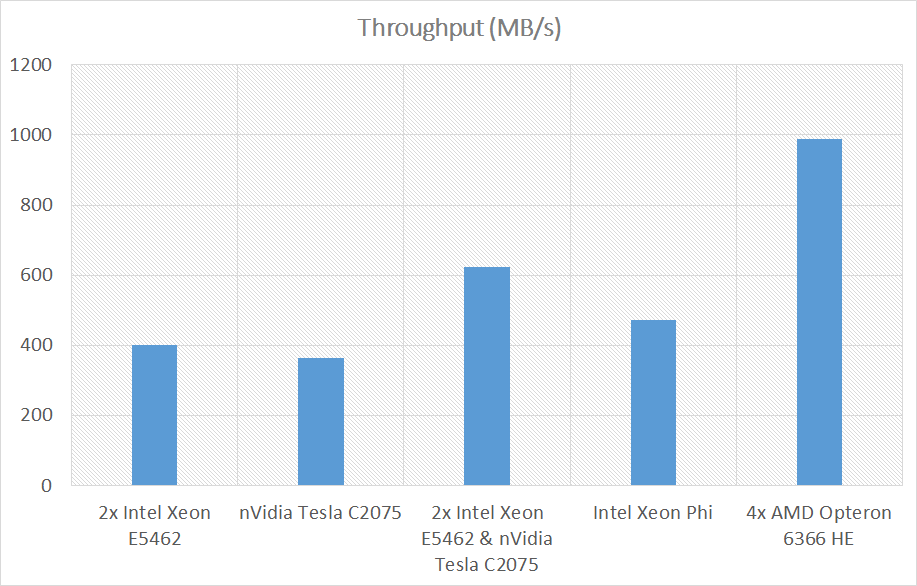
\includegraphics[width=\linewidth]{images/parsingScoringBest.png}
\caption{Parsing and Scoring Device Comparison}
\label{fig:parseScoringBest}
\end{figure}

\section{Discussion of Results}

\subsection{Data Transfer}

Data transfer rates between host and device are often a source of performance
issues when using accelerator chips. In the document classification system,
around 300MB is required to be transferred for each kernel invocation. Transfer
times, as measured during actual kernel executions, are around 110 milliseconds.

For the scoring only results, this is up to half of the total time spent to
score some documents. For instance the nVidia Tesla C2075 bloom filter
experiment has a scoring time is 232ms. This is a significant overhead. Given
that the PCI express bus speed was the original 1.0 specification with 4GB/s
maximum throughput, moving to a graphics card with similar compute performance,
but with PCI-E 3.0 capabilities would reduce the data transfer overhead to
around 30ms, improving overall time to 152ms, a reduction of around one third.

For the parsing and scoring results, the transfer time only represents at most
one fifth of the total time on the Intel Xeon Phi (The no bloom filter
experiment runs in 499ms). This is still a substantial overhead however, the
move to PCI-E 3.0 would only reduce this time to around 429ms, a throughput
improvement of around 16\%.

The simple reason behind the differences in effect of transfer rates on
performance between the scoring, and parsing and scoring code is that in the
latter, the OpenCL kernel spends more computational time on each byte of data
transferred. Both scoring, and parsing and scoring require a similar amount of
data to be transferred yet the latter does more work thus parsing and scoring on
the one device is the better option based on data transfer overhead alone. It is
also worth noting again that due to the speed of parsing on the C++ system being
low compared to the scoring speed, the improved data transfer rates will only
reduce latency in getting classification results back, but not improve
throughput overall given that the parser is the bottleneck.

\subsection{C++ versus OpenCL throughput}

Although the scoring only experiments on the CPU was initially purely for
reference, they also highlight a potential benefit of running a highly data
parallel algorithm on the CPU using OpenCL. The C++ version uses POSIX threads
to become multi-threaded and, with eight hardware threads, experience up to
7.82x better throughput compared to the single threaded version. This is as
expected, the maximum improvement is 8x however threading will inevitably result
in a bit of overhead. The surprise arrives when looking at the OpenCL version of
the scorer, it has around twice as high throughput compared to the multi-
threaded C++ version, thus making it nearly 20x quicker than the single threaded
version.

Looking at the results alone, this initially seems unusual however can be
explained. With POSIX threads, the document set is split evenly into eight sets,
one for each hardware thread. In terms of scheduling and memory access, this is
as granular as things go, each thread goes through its documents one by one. For
OpenCL, it has the same number of work items as there are documents. For the
TREC data set, this is around 77876 documents. OpenCL is free to schedule work
items on compute units allowing for more granular scheduling. This can enable
the runtime system to better hid memory access latency, resulting in the higher
throughput. Also, given that documents can be of different lengths, if a POSIX
thread has significantly longer documents than its counterparts, it will still
be working away while the others have finished. This can still happen on the
OpenCL system but with the granularity being significantly finer, it can be
mitigated.

\subsection{Effect of Bloom Filters}

The bloom filters were designed and added to the OpenCL kernel with the idea
that they will be able to save trips to the on-board memory for the GPU. With
GPUs having manual caching, the OpenCL kernel is responsible for moving the
bloom filter from global memory to local memory. The benefit of this is that the
bloom filter is guaranteed to be in the faster memory. This contrasts with the
CPU where the bloom filter can still bring benefit by migrating to L3 or L2
cache on the CPU but, since CPUs implement automatic caching, this is not
guaranteed to happen.

When a variable is moved in to cache, it isn't just that data value that is read
in, an entire cache line is read in. A cache line is typically on the order of
tens of bytes, with 64 bytes being the cache line size on all devices used. The
idea behind this is locality of reference, if a value at address x is read from,
it is likely the same process will need addresses near by in the near future.
The benefit of this is for the scoring only code, a read of one term, will read
in the next seven terms (8 terms are 64 bytes) into cache making subsequent
reads faster. This also benefits the parsing and scoring only code, a read of
one character will read in the next sixty three characters (64 characters are 64
bytes) making subsequent reads faster. This also holds true for GPUs as reads
from memory are done in chunks of around 64 bytes.

\subsubsection{Scoring Only}

Use of the bloom filter when running the scoring only code benefits almost all
devices, with the Intel Xeon Phi being the exception. Even on the single
threaded C++ code, a 26\% performance increase is observed in the best case (the
``no hits'' bloom filter). With a realistic application of the document
filtering being the case where most documents, and thus terms, are not of
interest to the classifier, the ``no hits'' bloom filter is not only the best
case, but is close to the average case as well.

Both the Intel and AMD CPU systems experience just over a factor of two increase
in performance when making use of the bloom filter in the best case. This is
strong evidence to suggest that the bloom filter is being moved into L3, or L2
cache and staying there for most of the kernel execution. This means the bloom
filter can be checked without going to primary memory, and if the bloom filter
returns a ``miss'' then the primary memory won't be read from at all.

The nVidia GPU has a modest performance increase of around 11\% with the normal
bloom filter, and 19\% in the best case. If one was to compare solely with the
CPU this may seem disappointing however the performance increase is still
significant, especially considering it's all from a 4KB buffer with little
computational overhead. Also, since there is no automatic caching, the benefit
of caching is limited by the memory model, and the kernel code itself.

The Intel Xeon Phi has peculiar results compared to the other device, the bloom
filter results in a performance drop of around 5\%. This is perhaps due to the
complicated cache mechanism required given the high number of independent cores.
Each code has its own, small L2 cache thus the bloom filter is unlikely to be
present in all of the cores simultaneously thus the potential benefit of the
bloom filter is small. It is possible for a single copy of data in cache to be
available for all cores, thus maximises cache capacity as the bloom filter is
only stored once, but this makes access significantly slower. Since
communication between cores and access to memory, is dictated by a ring
structure between cores, following a shortest distance algorithm
\footnote{\url{http://www.intel.co.uk/content/dam/www/public/us/en/documents/dat
asheets/xeon-phi-coprocessor-datasheet.pdf} Page 10}, this set up would appear
to be unsuitable for a bloom filter whose benefit relies on fast local access.

As discussed previously, the scoring code runs significantly faster on all
devices in comparison to the parser, thus it is the parser which is the system
bottleneck. Improvements in overall system performance can thus be obtained by
having the parsing and scoring executed on the same device.

\subsubsection{Parsing and Scoring}

Use of the bloom filter is a mixed bag of results when looking across different
devices. The Intel CPU benefits by up to 20\% in the best case whereas all other
single device runs experience a performance hit of as little as 5\% with the
Intel Xeon Phi to as much as 44\% with the AMD CPUs. Overall, the benefit is
reduced or mitigated entirely in comparison to the scoring only kernel.

Considering the Intel CPU system initially, it is the only system which still
has a performance improvement of up to 20\%. In the scoring code the performance
improvement exceeded 100\%. The bloom filter is used no more and no less than in
the scoring only code. The two primary reasons for this are related to the
amount of extra work in this kernel, and the extra variables required. As was
identified earlier, the parser is the bottleneck. This fact will remain true
even in this implementation which parses terms and scores them as soon as a full
term has been parsed. This means that, in terms of instruction count, a reduced
proportion is in the part of the code which would benefit from the bloom filter.
As such it is natural that, percentage wise, throughput will not improve as
much. The second relates to cache use itself. The scoring only code had very
little private variables; it read in a term, created three n-grams, had a few
variables to denote term range, score, and work item ID. This meant that less
cache space was being used by private variables, increasing the chance that the
bloom filter will not only migrate to CPU cache, but stay in cache for an
extended period of time. The parsing and scoring kernel has around twice as many
private variables, making fitting a bloom filter into the cache unlikely to be
possible for an extended period of time.

The AMD CPU experiences the biggest performance drop of nearly 50\%. This
contrasts heavily with the larger than 100\% increase in performance for scoring
only code. Everything discussed for the Intel CPUs is relevant to the AMD CPUs.
The AMD CPU has 16MB of L2 cache in comparison to the 12MB on the Intel CPUs
however, with the AMD CPUs core count being 16 compared to the Intel's count of
4, the amount of L2 cache per core is three times higher (3MB) on the Intel CPU
compared to the AMD CPU (1MB). This makes the situation of cache demand even
more severe and is likely to contribute to the heavy performance drop. The bloom
filter will be being read in regularly, removing other variables, just for those
variables to be read in shortly after, removing the bloom filter. This is
similar to the situation there primary memory and the swap space on disk are
continually being read from and written to. This is known as thrashing and is
responsible for significant drops of performance, similar to those experienced
by the AMD system.

The nVidia GPU experiences around a 20\% drop in performance in the best case by
using a bloom filter. Even with the GPUs local memory being under control of the
programmer, the extra demand of the local memory by the parser can have similar
effect as on the CPU. The extra variables will affect the occupancy of a compute
unit as less work items can be assigned simultaneously. The reduced number of
work items per compute unit could also be affecting the memory latency technique
effectiveness, resulting in the drop in performance.

The Intel Xeon again has around a 5\% performance drop, identical to the scoring
only version. With their being no difference in the bloom filter performance
change, the reasons discussed in the scoring only section are likely just as
valid for the parsing and scoring section.

In general, the bloom filter has a negative affect on most devices and could
easily be ignored in a real world implementation. Given that the Intel CPU
has some benefit from a bloom filter, it could still be beneficial to try the
bloom filter on the target system as a performance benefit on some devices is
evidently still applicable.

\subsection{Overall}

In previous work, the parser was running on the CPU at 427MB/s
\cite{HybridCPUFPGA} and was the bottleneck of the system when scoring was
conducted on an FPGA. This is also true with the GPU however, if both the CPU
and GPU are parsing and scoring their own set of documents, it is possible to
achieve in excess of 620MB/s, around a 45\% increase in performance on a fairly
typical two CPU and one GPU system. In comparison to the CPU and GPU results
individually, there is only around a 15\% overhead when running the devices in
parallel. Most of this overhead comes from the CPU time required to detect the
beginnings of documents before sending the data off to the OpenCL device. If the
CPU was used solely to read in documents from a network feed and work out the
locations of document beginnings, it's likely the case that in a multi-GPU set
up, the GPUs could each be used to parse and score, with the CPU host having
plenty of cycles free to coordinate the system. Also, the PCI-E bandwidth is
unlikely to be a bottleneck as the GPUs can be transferring data and executing
kernels at slightly different times meaning a multi-GPU set up is unlikely to
have significant overhead and scale almost linearly with the number of devices.
This can be shown in the dual Intel Xeon Phi runs, which experience a near
linear increase (80\%) compared to the single Intel Xeon Phi. This is with both
devices requirement documents at the same time, and would represent the worst
case in a real life application. In reality, the devices would be at different
stages of classification meaning CPU cycles are more likely to be used more
evenly over a set time frame, rather than bursts of high activity, followed by
period of little activity while both devices are parsing and scoring.
